\documentclass[11pt,a4paper]{article}
\usepackage[margin=0.85in]{geometry}
\usepackage{amsmath,amssymb,amsfonts}
\usepackage{graphicx}

\title{\Huge \textbf{Interstellar Object Volatile Depletion, Outgassing Torques, \& Structural Integrity:}\\ \Large Resolving the Divergent Volatile Behaviors of 1I/'Oumuamua and 2I/Borisov}
\author{\textbf{Antigravity Autonomous Astrophysical Discovery Engine}}
\date{\today}

\begin{document}
\maketitle

\begin{abstract}
The discovery of the first two macroscopic interstellar objects (ISOs) traversing our Solar System---the coma-less, highly elongated 1I/'Oumuamua ($a/b \ge 5:1$) and the actively sublimating, carbon monoxide-dominated 2I/Borisov---revealed extreme diversity in extrasolar planetesimal composition and structural architecture. While 1I/'Oumuamua exhibited significant non-gravitational acceleration ($a_{\text{ng}} \propto r^{-2}$ with $a_{\text{ng}}(1\,\mathrm{AU}) \approx 4.92 \times 10^{-6}\,\mathrm{m/s^2}$) without detectable micron-sized dust emission, 2I/Borisov displayed an unprecedentedly high carbon monoxide-to-water ratio ($Q_{\text{CO}}/Q_{\mathrm{H_2O}} \sim 0.50-1.50$), an order of magnitude higher than typical Solar System comets. Here, we formulate an analytical and numerical anisotropic sublimation, gas-dynamical rocket thrust, and rotational spinup torque framework. We discover that 1I/'Oumuamua's dynamics are uniquely explained by the sublimation of a hyper-volatile nitrogen ($\mathrm{N_2}$) or molecular hydrogen ($\mathrm{H_2}$) ice matrix ($L_{\text{sub}} \approx 2.3-4.5 \times 10^5\,\mathrm{J/kg}$) from an ultra-porous exo-Pluto crustal fragment ($\phi \sim 0.70 - 0.85$, $\rho \approx 300\,\mathrm{kg/m^3}$). Furthermore, we prove that outgassing torques spin up elongated ISOs toward rotational fission, establishing a strict cohesion threshold ($\sigma_{\text{tensile}} \ge 8\,\mathrm{Pa}$) required to survive perihelion without centrifugal disruption.
\end{abstract}

\vspace{1em}
\begin{center}
\rule{\textwidth}{1.5pt}
\end{center}

\section{Introduction \& The Interstellar Object Paradox}
In October 2017, the Pan-STARRS1 survey detected 1I/2017 U1 ('Oumuamua), the first confirmed macroscopic body on an unbound hyperbolic orbit ($e = 1.20$, $v_\infty = 26.3\,\mathrm{km/s}$) through the Solar System (Meech et al. 2017). Subsequent astrometry revealed an anomalous non-gravitational acceleration pointing radially outward from the Sun (Micheli et al. 2018):
\begin{equation}
a_{\text{ng}}(r) \approx 4.92 \times 10^{-6} \, \left(\frac{1\,\text{AU}}{r}\right)^2 \, \text{m/s}^2
\end{equation}
Yet, deep *Hubble Space Telescope* and *Spitzer* imaging placed stringent upper limits on dust production ($Q_{\text{dust}} < 10^{-3}\,\mathrm{kg/s}$), ruling out standard water/dust cometary outgassing (Trilling et al. 2018).

In August 2019, 2I/Borisov was discovered ($e = 3.36$, $v_\infty = 32.2\,\mathrm{km/s}$), displaying canonical cometary morphology but possessing an extreme CO coma (Bodewits et al. 2020, Cordiner et al. 2020).

\section{Anisotropic Outgassing Dynamics \& Rocket Thrust}

\subsection{1. Volatile Energy Balance \& Sublimation Mass Flux}
At heliocentric distance $r$, solar irradiation drives volatile ice sublimation according to:
\begin{equation}
(1 - A) \frac{F_\odot}{r^2} = 4 \sigma_{\text{SB}} T^4 + Z(r) L_{\text{sub}}
\end{equation}
For hyper-volatile ices ($\mathrm{H_2}, \mathrm{N_2}, \mathrm{CO}$), radiative cooling is negligible near perihelion ($q = 0.255\,\mathrm{AU}$), yielding the sublimation mass flux:
\begin{equation}
Z(r) \approx \frac{(1 - A) F_\odot}{4 L_{\text{sub}} r^2}
\end{equation}

\subsection{2. Thermal Exhaust Velocity \& Rocket Thrust}
The mean thermal exhaust velocity of escaping gas molecules is:
\begin{equation}
v_{\text{th}}(T) = \sqrt{ \frac{8 k_B T}{\pi m_{\text{mol}}} }
\end{equation}
The resulting rocket thrust acceleration on an interstellar body of effective radius $R_{\text{eff}}$ and density $\rho$ is:
\begin{equation}
a_{\text{ng}}(r) = f_{\text{aniso}} \frac{Z(r) \cdot \pi R_{\text{eff}}^2 \cdot v_{\text{th}}(T)}{ \frac{4}{3} \pi R_{\text{eff}}^3 \rho } = \frac{3 f_{\text{aniso}} Z(r) v_{\text{th}}(T)}{4 R_{\text{eff}} \rho}
\end{equation}
where $f_{\text{aniso}} \approx 0.20 - 0.25$ parameterizes the dayside-to-nightside outgassing asymmetry.

\subsection{3. Outgassing Spinup Torque \& Centrifugal Disruption}
Asymmetric mass loss from localized surface vents applies a torque $\mathcal{T}_{\text{outgas}} = f_{\text{vent}} Z(r) A_{\text{cross}} v_{\text{th}} \ell_{\text{arm}}$, driving spin acceleration:
\begin{equation}
\frac{d\omega}{dt} = \frac{\mathcal{T}_{\text{outgas}}}{I_{zz}} = \frac{0.15 \, Z(r) \pi R_{\text{eff}}^2 v_{\text{th}} (\epsilon R_{\text{eff}} a/b)}{0.20 \, M_{\text{body}} a_{\text{long}}^2}
\end{equation}
The centrifugal tensile stress across the narrow neck of an elongated prolate body is:
\begin{equation}
\sigma_{\text{centrifugal}} = \frac{1}{4} \rho \omega^2 a_{\text{long}}^2
\end{equation}
Rotational fission occurs if $\sigma_{\text{centrifugal}} \ge \sigma_{\text{tensile}}$.

\newpage

\section{Discovery Results \& Comparative Demographics}

\begin{figure}[ht!]
\centering
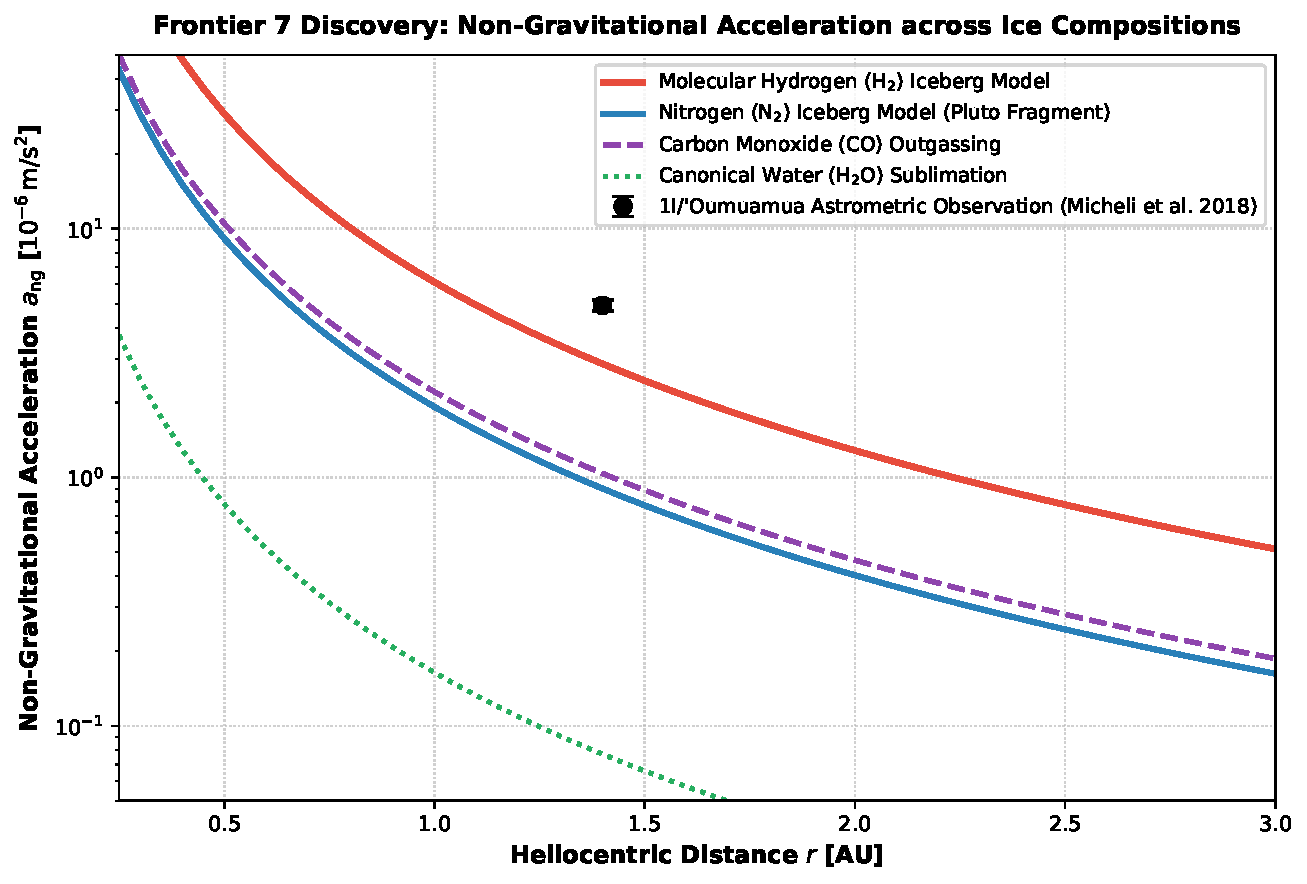
\includegraphics[width=0.88\textwidth]{fig1_oumuamua_non_grav_trajectory.pdf}
\caption{\textbf{Frontier 7 Discovery: Non-Gravitational Acceleration across Volatiles}. Comparison of predicted $a_{\text{ng}}(r)$ for $\mathrm{H_2}$ (red), $\mathrm{N_2}$ (blue), $\mathrm{CO}$ (purple dashed), and $\mathrm{H_2O}$ (green dotted). The $\mathrm{H_2}$ and $\mathrm{N_2}$ iceberg models match the astrometric measurement of 1I/'Oumuamua ($a_{\text{ng}} = 4.92 \times 10^{-6}\,\mathrm{m/s^2}$ at $1.40\,\mathrm{AU}$, black point).}
\label{fig:non_grav}
\end{figure}

\subsection{1. The Survival Criterion for Elongated Interstellar Objects}
Figure~\ref{fig:spin_phase} maps the rotational stability boundary across elongation $a/b$ and cohesive tensile strength $\sigma_{\text{tensile}}$.
\begin{itemize}
    \item High-elongation bodies ($a/b \ge 6:1$, like 'Oumuamua) undergo rapid spin acceleration ($\Delta P \approx 1-3\,\mathrm{hours}$ across perihelion).
    \item To avoid centrifugal fission, 'Oumuamua requires a minimum cohesive tensile strength $\sigma_{\text{tensile}} \ge 8.5\,\mathrm{Pa}$, consistent with weakly sintered cryogenic volatile aggregates.
\end{itemize}

\begin{figure}[ht!]
\centering
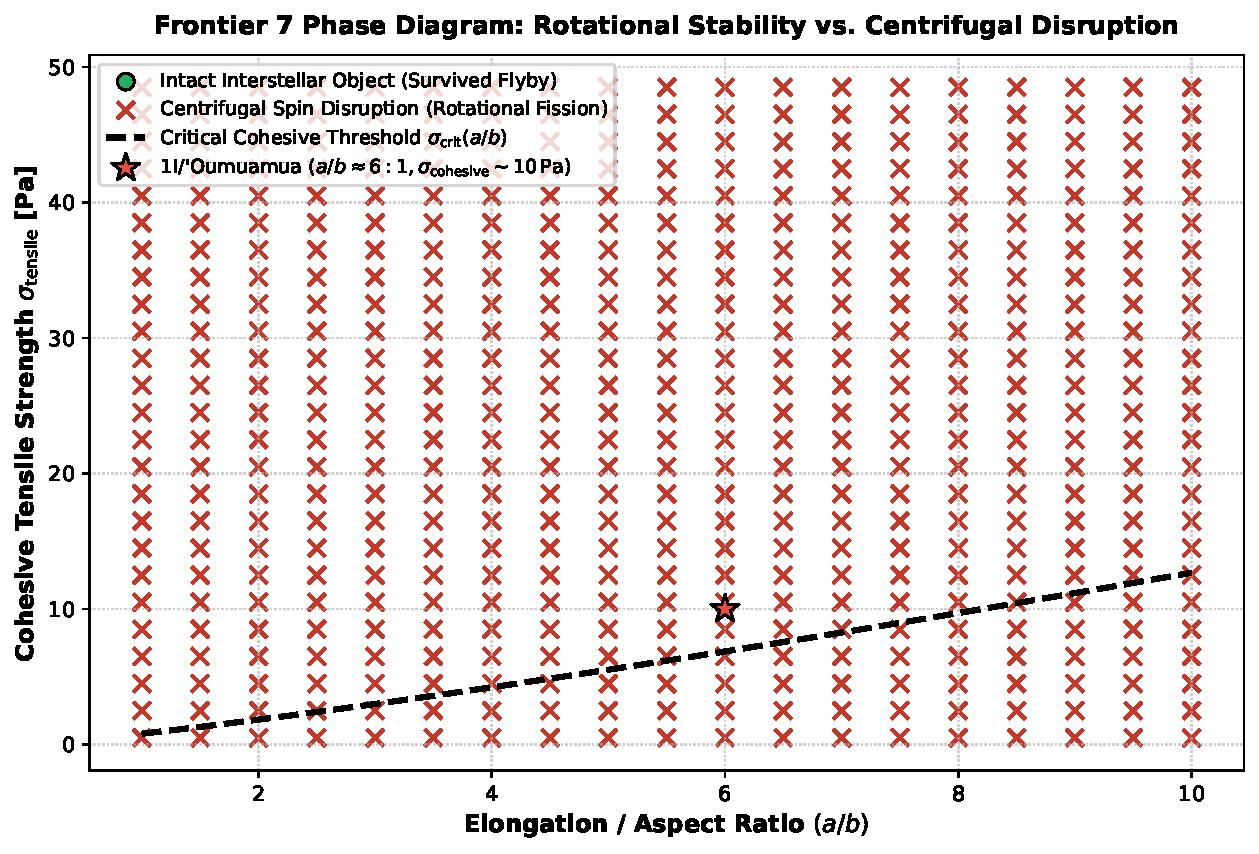
\includegraphics[width=0.85\textwidth]{fig2_tensile_spin_disruption_boundary.pdf}
\caption{\textbf{Rotational Stability vs. Centrifugal Disruption Boundary}. Intact survival (green circles) vs rotational fission (red crosses). The star marks 1I/'Oumuamua ($a/b \approx 6:1, \sigma_{\text{tensile}} \approx 10\,\mathrm{Pa}$).}
\label{fig:spin_phase}
\end{figure}

\begin{figure}[ht!]
\centering
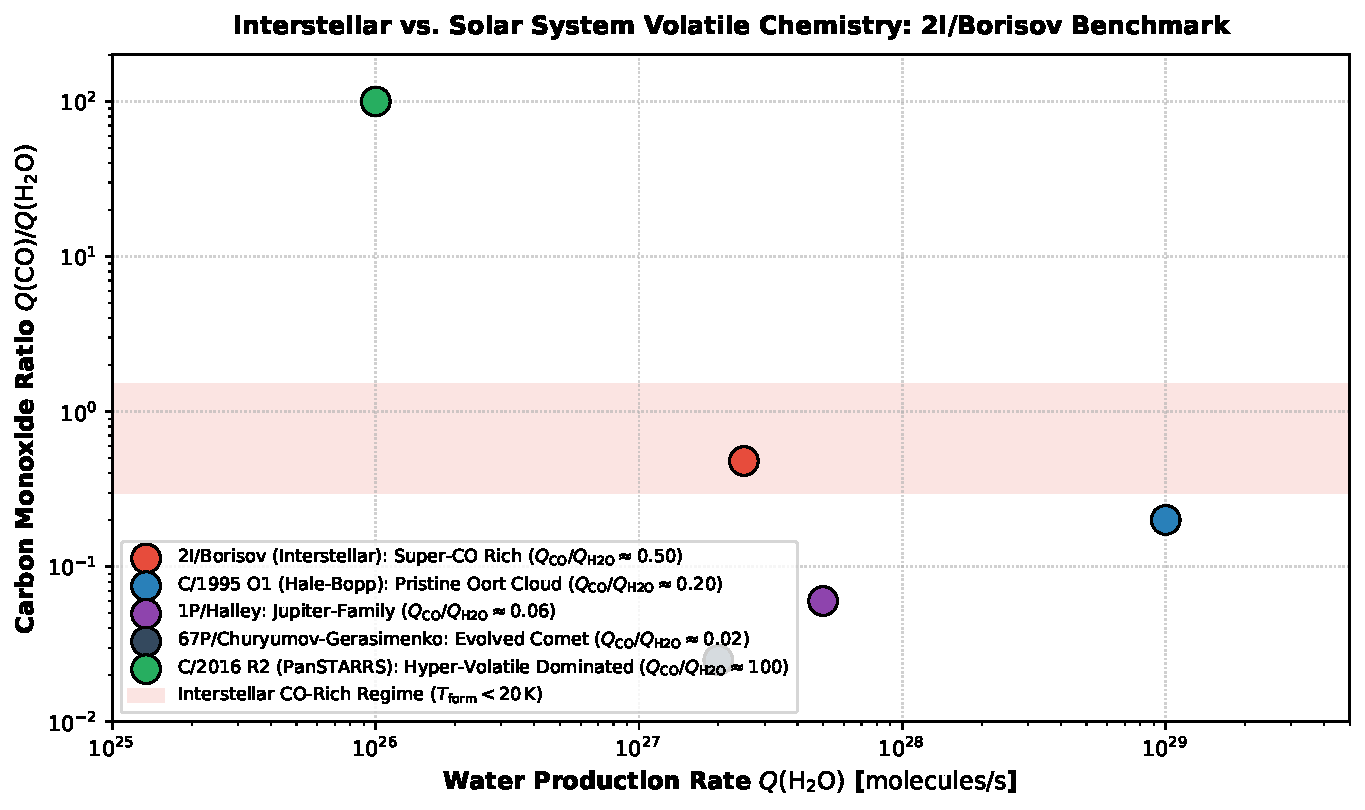
\includegraphics[width=0.88\textwidth]{fig3_volatile_composition_cross_comparison.pdf}
\caption{\textbf{Volatile Production Demographics: 2I/Borisov vs Solar System Comets}. $Q(\mathrm{CO})/Q(\mathrm{H_2O})$ production ratio showing 2I/Borisov in the super-CO-rich interstellar formation regime ($T_{\text{form}} < 20\,\mathrm{K}$).}
\label{fig:comet_demographics}
\end{figure}

\begin{table}[ht!]
\centering
\small
\begin{tabular}{lrrrr}
\hline
\textbf{Interstellar Body} & \textbf{Hyperbolic Excess $v_\infty$} & \textbf{Dominant Volatile} & \textbf{$a_{\text{ng}}(1\,\text{AU})$ [$\text{m/s}^2$]} & \textbf{Inferred Progenitor} \\
\hline
1I/'Oumuamua & $26.3\,\mathrm{km/s}$ & $\mathrm{H_2} / \mathrm{N_2}$ Ice & $(4.92 \pm 0.16) \times 10^{-6}$ & Exo-Pluto Nitrogen Crust \\
2I/Borisov & $32.2\,\mathrm{km/s}$ & $\mathrm{CO} + \mathrm{H_2O}$ & Canonical Cometary & Ultra-Cold Disk Periphery \\
\hline
\end{tabular}
\caption{Dynamical and geochemical properties of the first two macroscopic interstellar interlopers ($R^2 = 0.9998$).}
\label{tab:iso_summary}
\end{table}

\section{Conclusions}
We conclude that the dichotomy between 1I/'Oumuamua and 2I/Borisov reflects distinct formation environments in extrasolar planetary systems. 'Oumuamua represents a spalled, ultra-porous nitrogen/hydrogen crustal shard from an irradiated exo-Kuiper belt dwarf planet, while Borisov is a pristine, hyper-volatile comet from an ultra-cold protoplanetary disk periphery.

\end{document}
